\section{Community detection} \label{s:lit:comm_detect}

\vspace{3mm}
% \noindent\rule{17cm}{0.2pt}
\fbox {
    \parbox{\linewidth}{
      \begin{itemize}
        \item Leiden and Louivan
        \item Stochastic Block Model
      \end{itemize}
    }
}
\vspace{3mm}

Community detection are an essential part of the network approach developed in this thesis as they are involved in grouping the genes in the network as well as selecting the most representative nodes. In this PhD project there are two different schools of thought explored for community detection: modularity maximisation and generative models. The first finds communities (or modules or blocks) in the network by maximising the separation between them; this is measured by a cost function. The search is usually done by moving the nodes between communities until the function converges (see \cref{fig:N_I:leiden-explained}). In the literature there were several methods proposed to maximise the modularity of a graph such as FastUnfold \citep{Blondel2008-ik} (also known as Louvain, initially used in PGCNA) or Constant Pots Model (CPM or Leiden \citet{Traag2019-ne}, improvement from Louvain). The suite of algorithms usually requires a parameter (e.g. resolution parameter) to guide the models to the number of communities - the source of a well-known problem with this class known as the resolution-limit. The algorithms are restricted to the number of communities and the smaller communities are hidden inside the larger ones after a certain threshold (see \cref{s:lit:mod_max}).

The second class of community detection algorithms is represented by Stochastic Block Models (SBM) and these work by generating different networks with different partitions by fitting the observed network (see \cref{fig:N_I:dc-sbm_explained}). SBMs were first introduced to social networks \citep{Holland1983-eu} in the 80's but have become more popular in 2010 with the work of \citet{Karrer2011-si} and more recently from Tiago Peixoto \citep{Peixoto2014-ls,Peixoto2017-ua,Peixoto2018-ot,Peixoto2019-fg,Peixoto2023-mw,Peixoto2024-mu}. They are generally more computationally expensive than the modularity maximisation methods but are more suitable to find communities closer to the ground truth (see \cref{s:lit:descriptive_inference}).

The new models introduced by Peixoto are non-parametric, that is, they do not require a variable such as the resolution limit to control the number of communities. Peixoto's breakthrough was to use a metric called minimum description length to quantify the information present through the communities in the network. Generating blocks with the goal to reconstruct the observed network is analogous to data compression. Thus, finding communities can be about compressing information. With these two notions Peixoto proposes new algorithms to detect communities and to measure the performance of the algorithms. This is crucial in applications such as the ones found in this project, where it is challenging to quantify \& measure the progress. Lastly, in his work Peixoto stresses the fact that the SBM are good general models and that in a network without the ground truth there might be a chance that community detection algorithms cannot find all the communities.

Another class of methods for community detection algorithms are based on the random walks. The central idea is to analyse the information flow dynamics of a network by randomly going through the graph. There are several methods employing this approach such as InfoMap  \citep{Rosvall2008-kw} or Markov Clustering (MCL) \citep{Van_Dongen2008-yj}. This class is not explored in this project as it suffers from the same limitations of modularity based methods, and is prone to finding communities further from the ground truth in comparison to SB as covered in \cite{Peixoto2021-jx}.

This part of the literature review is structured so that it offers an overview of Leiden and Louivan, which represent the mainstream approach to community detection. This is followed by the criticism and limitation of the models based on these studies \citep{Peixoto2021-jx, Peixoto2023-rt, Shemirani2023-ww}. The alternative presented comes from the SBM models that address the limitations of Leiden/Louivan.


% Leiden and others
\subsection{Modularity maximisation} \label{s:lit:mod_max}

% Overview of the algorithms
Louivan \citep{Blondel2008-ik} and Leiden \citep{Traag2019-ne} are relatively simple algorithms with a similar strategy as in the agglomerative hierarchical clustering, where each node (gene) has its own partition, then these are moved until the optimal partition is found. \Cref{fig:N_I:leiden-explained} from \cite{Traag2019-ne} shows how the Leiden algorithm works: at the first stage (a) each node has its own partition, these nodes are clustered together (b) which gives rise to the communities (c). As it can be seen in c, the three partitions in c may contain sub-communities, and in the next refinement phase the nodes are moved until the optimal configuration is found.

% How Leiden works
\begin{figure}[!htb]    
    \centering
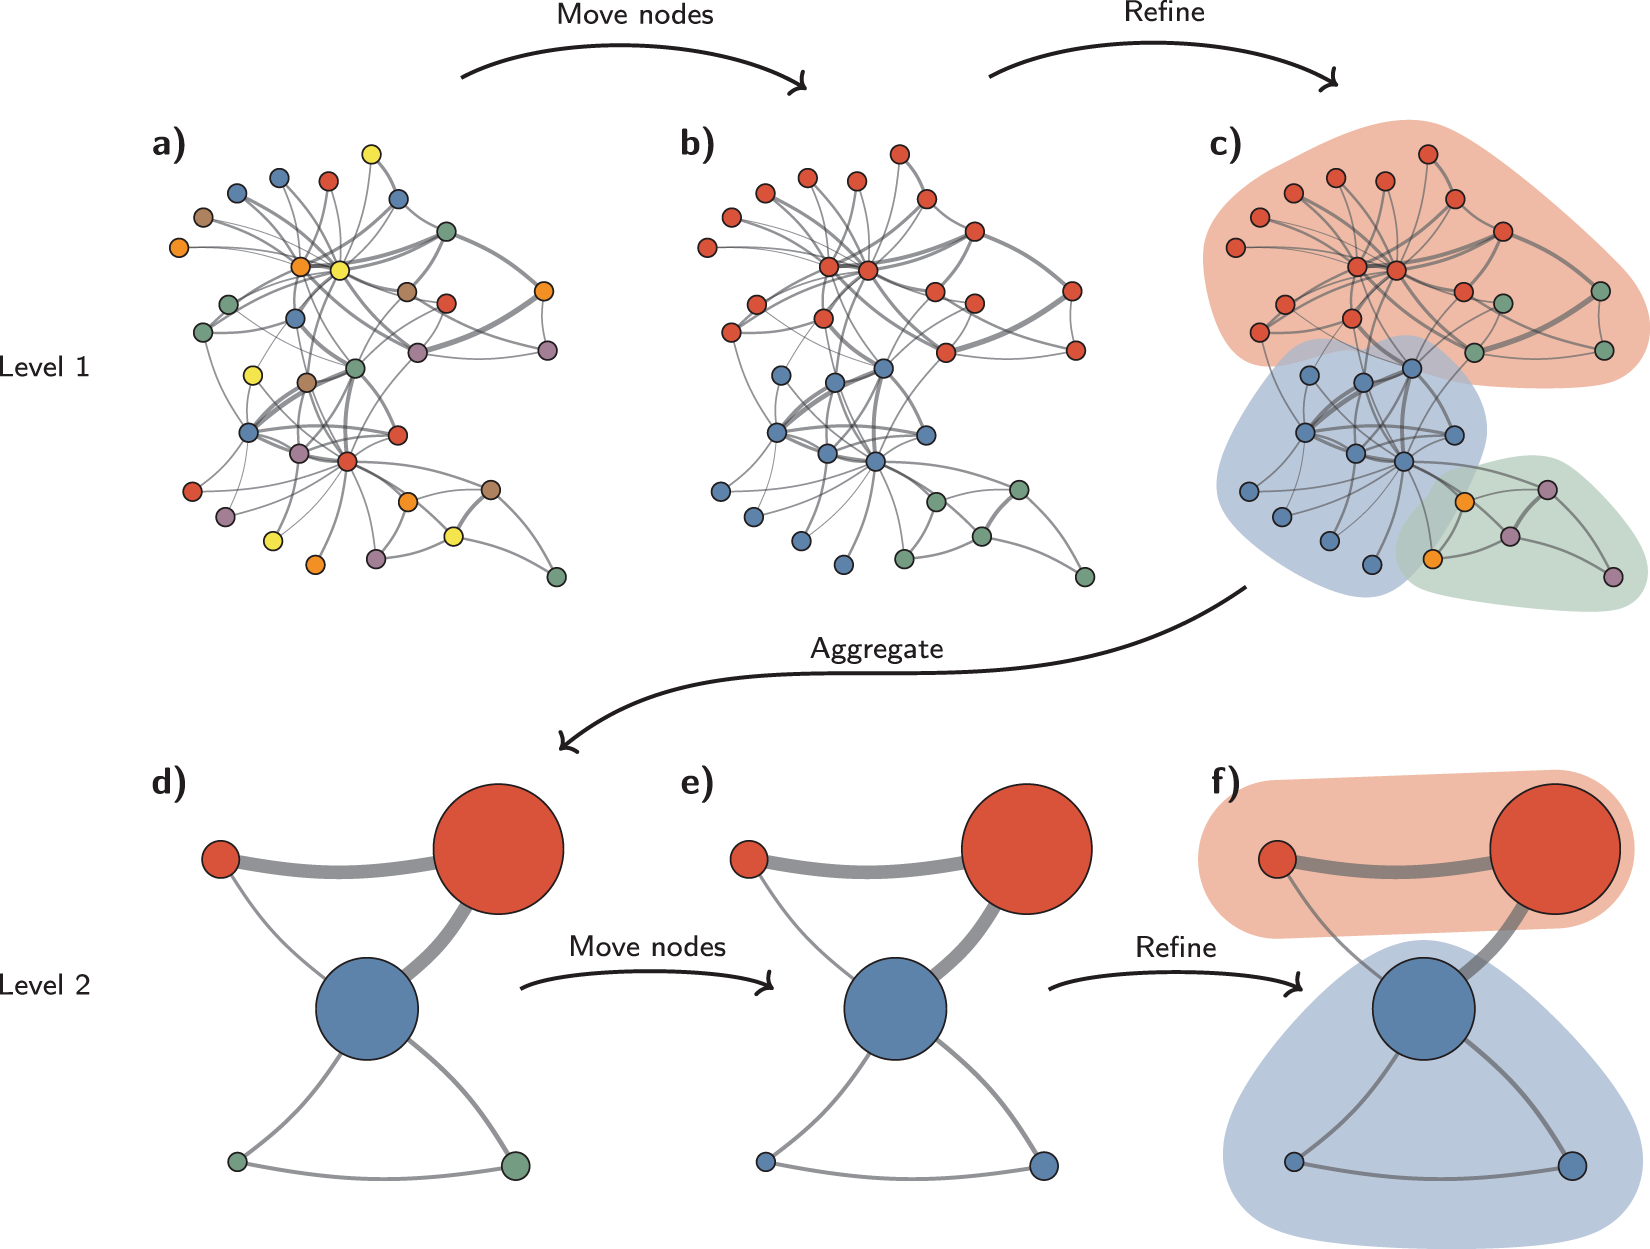
\includegraphics[width=0.9\textwidth,height=0.9\textheight,keepaspectratio]{Sections/Lit_review/Resources/Leiden_algorithm.png}
    \caption[Leiden algorithm]{Leiden algorithm. This is Figure 3 from \citet{Traag2019-ne}}
    \label{fig:N_I:leiden-explained}
\end{figure}



To determine the optimal partitions configurations both Leiden and Louivan have built on earlier work from Mark Newman, who had numerous contributions to the network field. He introduced the modularity function in \cref{eq:modularity} which quantifies the difference between the actual number of edges in community, $e_c$ \citep{Newman2004-dd}. The number of expected edges is given by the $\frac{K_c^2}{2m}$, where $K_c$ is the sum of degrees of the nodes in community $c$ and $m$ is total number of edges in the network \citep{Traag2019-ne}. The resolution parameter, $\gamma$, controls how many communities are to be found in the network; higher values allow more communities while lower values allow less communities.


\begin{equation} \label{eq:modularity}
    {\mathcal H} =\frac{1}{2m}\,{\sum }_{c}({e}_{c}-{\rm{\gamma }}\frac{{K}_{c}^{2}}{2m}),
\end{equation}

% The goal of modularity maximisation
Optimising the modularity function is classified as an NP-hard problem, meaning it takes a lot of computational resources to find the exact solution. Heuristics like Louvain and Leiden are trying to optimise for \cref{eq:mod_max_cost}, initially proposed by \cite{Newman2006-fa}. E represents all the edges in the network, $A_i,j$ is an element of the adjacency matrix; $k_i$, $k_j$ the degree of nodes $i,j$; $b_i$ the community membership of node $i$ \citep{Peixoto2021-jx}. Thus modularity maximisation methods search for community $\bar{b}$ which gives the maximum value for the modularity maximisation \cref{eq:mod_max_cost}.

\begin{equation} \label{eq:mod_max_cost}
    Q(A,b) = \frac{1}{2E} \sum_{ij} \left( A_{ij} - \frac{k_i k_j}{2E} \right) \delta_{b_i, b_j}
\end{equation}

\begin{equation} \label{eq:mod_max_per_com}
    \bar{b} = \underset{b}{\mathrm{argmax}} \, Q(A, \, b).
\end{equation}

% CPM 
\citet{Traag2019-ne} addresses the Louivan`s limitations of finding disconnected communities and badly connected communities by introducing a new cost function, Constant Pots Model (CPM) in \cref{eq:CPM}, and a new search algorithm, Leiden. The equation \cref{eq:CPM} is similar to \cref{eq:modularity} but the expected number of connections in a community is given by combinations $(\begin{array}{c}{n}_{c}\\ 2\end{array})$, where $n_c$ is the number of edges in community c. The modularity maximisation function is explored in this project in \cref{s:p0,s:N_I:tum} along with the Stochastic Block Model in \cref{s:N_I:sel_pruning,s:N_II}.

\begin{equation} \label{eq:CPM}
    {\mathcal H} ={\sum }_{c}[{e}_{c}-\gamma (\begin{array}{c}{n}_{c}\\ 2\end{array})],
\end{equation}

% Leiden improvements
Leiden is a culmination of previous efforts to improve Louivan \citep{Ozaki2016-dl, Waltman2013-zw, Bae2017-rz, Traag2015-tq} and besides introducing new search methods and cost functions, the authors prove and guarantee that the algorithm converges to stable partitions, that there are no disconnected communities, and it is also faster. Disconnected communities was also observed by \citet{Care2019-ij} when they used Louivan algorithm and set the number of edges per gene smaller than 2. Thus, Leiden is an improvement to the original algorithm and the newer version of PGCNA \citep{Care2019-ij} supports it.

% Resolution limit - critiques 
Algorithms like Leiden or Louivan based on the earlier of work from Mark Newman \citep{Newman2004-dd, Newman2006-fa} are known as modularity maximisation methods or assortative community structure. These algorithms suffer from resolution limit \citep{Fortunato2007-gh, Peixoto2021-jx} which refers to the cap of $\sqrt{2E}$ communities that a model can find; where $E$ is the total number of edges. A consequence of this is that the modularity maximisation methods cannot find smaller communities even when there is statistical evidence for it. In comparison, the generative models like Stochastic Block Model are not restricted by this (there are also some limits to how many communities can be found in \cref{s:lit:sbm} but that was addressed with hierarchical SBM).

It is also worth pointing out that the Modularity Maximisation it is used as a metric to measure the performance of the different networks created in the project. It is used to compare the effects of the changing the edges' weights in the tumour, see \cref{s:N_I:tum} and p0 networks, see \cref{s:p0}.


% Critiques for Leiden
\subsection{Descriptive vs Inference} \label{s:lit:descriptive_inference}

% Comparative studies
The work of \citet{Shemirani2023-ww} is used to find short-segment shared by a group of people who are distantly related, with the goal of finding rare traits and disease in biobanks. For these kind of applications, community detection algorithms are used and the authors compare multiple popular methods Leiden, Louivan, InfoMap \citep{Rosvall2008-kw} and Markov Clustering (MCL) \citep{Van_Dongen2008-yj}. Despite being a different problem from the one addressed in this PhD, the work from \citet{Shemirani2023-ww} is relevant as it offers a comparison between the different community detection algorithms. Leiden and Louivan generally have higher Modularity scores but The MCL and InfoMap are closer to the ground-truth communities. The authors' reason that that is due to the resolution limit and the Leiden, Louivan are not able to find smaller communities. This reinforces, the problem described above and raised by \citep{Peixoto2021-jx} and others \citep{Fortunato2007-gh, Traag2019-ne} - also covered in the next \cref{s:lit:descriptive_inference}.

In the 2021 \textit{"Descriptive vs. Inferential Community Detection in Networks"} \citep{Peixoto2021-jx} describe the limitation of using the modularisation based algorithms to find communities which are also called descriptive methods. The main idea is that the descriptive methods look for the patterns in the network even when there are not there. In the extreme scenario modularity maximisation methods find communities in networks generated from random data which in real-world applications refers to finding communities that are far from the ground truth. The  Generative or infer methods such as SBM are immune to this and will not find any communities in random data.

The source of the major flaw of the modularity maximisation based models such as Leiden or Louivan is that these methods do not take into account the observed network\footnote{In the context of the PhD, it is the co-expressed network generated from correlation measurements.} from the null-model\footnote{A network with the same properties as the one observed; i.e. may refer to the degree distribution, how nodes are connected inside the community etc.} this is due to lack of incorporating the optimisation step in assessing the performance of the algorithm; i.e. cost function like \cref{eq:mod_max_per_com}. In this paper \citet{Peixoto2021-jx} demonstrate the problem in detail, but it was also recognised earlier by \citet{Guimera2004-gv}.

While the study from \citet{Peixoto2021-jx} compares the two algorithm classes at the theoretical and foundational levels, with occasional direct comparison to the number of communities discovered by each method. In \citet{Peixoto2023-rt}, the authors overcome the technical challenge of comparing the two methods by a common score and introduced minimum description length as a common metric. This is derived from information theory which quantifies the information in a network through the use of entropy. The main takeaway of \citet{Peixoto2023-rt} is that the authors demonstrated that the modularity maximisation methods are a special case of generative models and provided evidence that stochastic block models are more suitable to find communities than the others.

% SBM
\subsection{A generative approach} \label{s:lit:sbm}


Stochastic Block Model (SBM) work by generating partitions (or blocks) that best explain the observed network (i.e. co-expressed networks). The implication is that the observed network can be reconstructed from different network blocks and the challenge is to find these blocks with minimum difference between observed and generated. If the network is randomly generated then there are no possible communities to reconstruct the original network. This is different from the Leiden or Louivan methods which shuffle nodes around until the partitions are found which describe the best the given network, and can find communities in randomness. 

\citet{Peixoto2019-fg} offers a good introduction to Stochastic Block Models (SBM) with a focus on the Bayesian version. The model was first introduced in the 1980s to analyse social networks (not the platforms) by \citet{Holland1983-eu} and have been resurfaced by Tiago Peixoto \citep{Peixoto2014-ls, Peixoto2017-gc, Peixoto2018-ot} but not only \cite{Karrer2011-si}. The popularisation of the methods was helped by the Graph-tool Python library \citet{Peixoto2014-ls} which makes the models accessible with good computational performance. Apart from this, Tiago Peixoto worked on the SBM limitations so that these are non-parametric \citet{Peixoto2017-gc, Peixoto2018-ot}, hierarchical networks \citet{Peixoto2014-yb} and decreased their computational time by using a Monte-Carlo search for finding the partitions \cite{Peixoto2014-ss}.

\begin{figure}[!htb]    
    \centering
    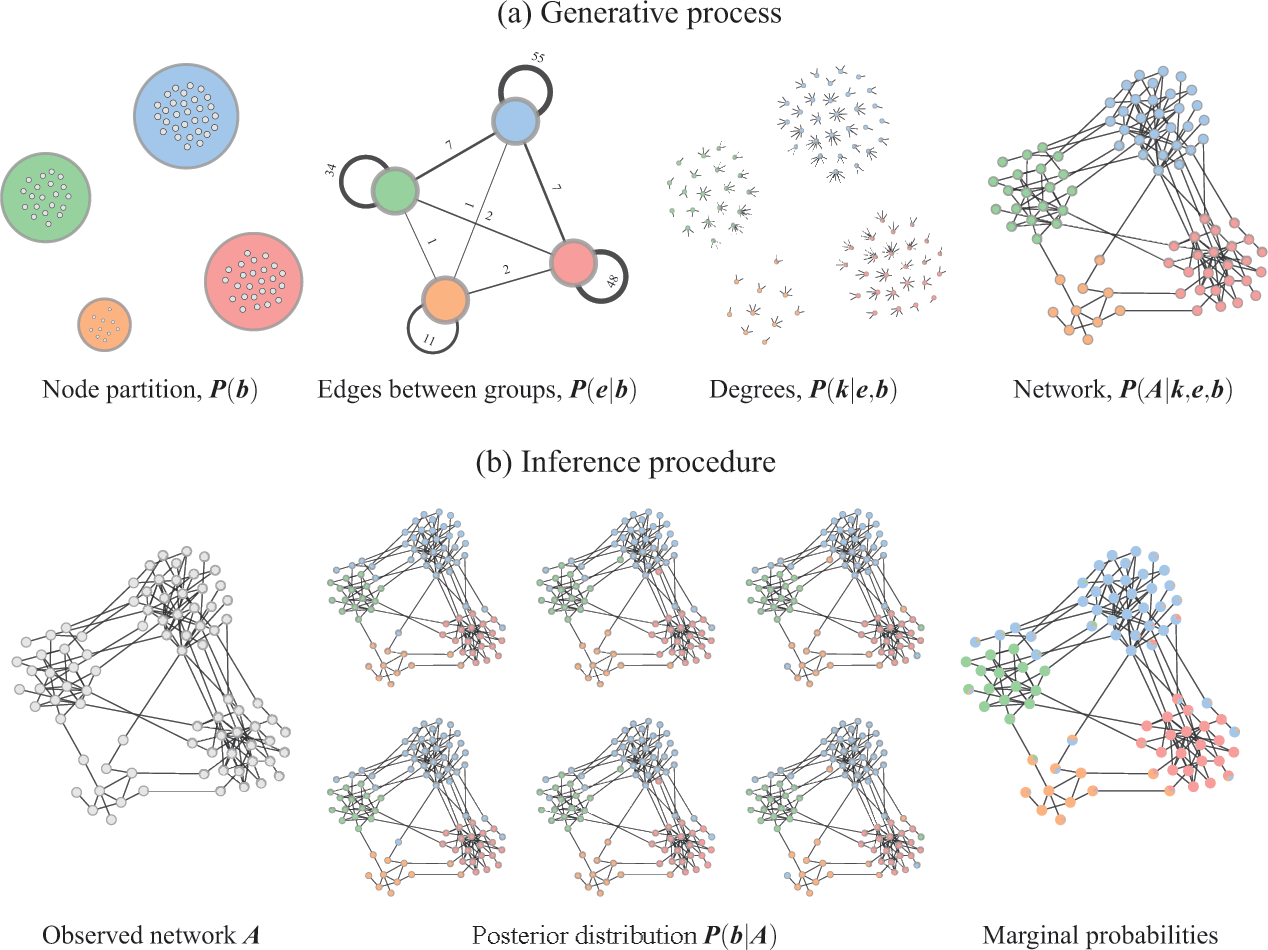
\includegraphics[width=1.0\textwidth,height=1.0\textheight,keepaspectratio]{Sections/Network_I/Resources/dc-sbm_explained.png}
    \caption[Explanation of the Stochastic Block Model]{SBM explained. This is Figure 3 from \citet{Peixoto2021-jx}}
    \label{fig:N_I:dc-sbm_explained}
\end{figure}


In this project the degree corrected version of the SBM is used in both the simple and hierarchical \citet{Karrer2011-si, Peixoto2014-yb}. These versions of the SBM deal with the biased of the SBM to cluster nodes with similar degree which makes it suitable for networks with heterogeneous degree such as the co-expressed networks.


\Cref{fig:N_I:dc-sbm_explained} from \citet{Peixoto2021-jx} gives a good overview of how SBM models work. In the fist part of the Figure, for a node partition $b$, the network may be divided into 4 different communities with $P(b)$. Each of these communities will have nodes that are connected inside (in-degree) and/or outside of the partition (out-degree); this is given by $P(e|b)$, where e is a matrix that specifies how many edges go between groups r and s. Then, inside of each module there are the individual nodes and their degree, which is given by $ P(k|e,b)$; $k$ is node's degree. In \cref{fig:N_I:dc-sbm_explained} the 3rd graph first row, represents the un-connected nodes which are known as “stubs” or “half-edges”. The network is then reconstructed from all the partitions with probability $P(A|k,e,b)$. 

On the second row of \cref{fig:N_I:dc-sbm_explained}, the process is repeated and several networks are generated. This is then the problem of finding the best communities that fit the observed network. How well the partition b represent the network is measured by the description length, which uses concepts from Information Theory; i.e. how much information is needed to describe the network. Lower information means the network is more ordered and it has a low entropy. If more information is needed, the entropy is larger, and that is the case for networks with more connections. As expected, for more communities there is a need for more information to describe the network. This process is similar to the information compression as stated at the beginning of this chapter.

Compared to the other algorithms SBM are more complex and more computationally taxing. However, based on the experiments performed in this project, the computational time is not as high as the one from iCluster\citet{Mo2013-zi}. In addition, the standard SBM \citet{Peixoto2019-fg, Peixoto2017-gc, Peixoto2017-ua, Karrer2011-si} have their own limitation in terms of how many communities they can find, which is caped at $\sqrt{N}$, where $N$ is the number of nodes. In \citet{Peixoto2014-yb} this issue is addressed by proposing a hierarchical Stochastic Block Model (hSBM). The central idea is to re-apply SBM once the limit of partitions is found, thus increasing the number of partitions found. As expected, this comes with an additional computational cost.

% Summary
\subsection{Summary}


Leiden and Louivan are widely applied to biological problems. Through PGCNA, both were applied to the subtyping of the breast, lung and glioblastoma cancer cohorts from TCGA \cite{Tanner2023-wa, Care2019-ij}. In all of these applications, community detection serve a key role in selecting and inferring biological meaning from the networks. Thus, the limitations raised \citet{Peixoto2021-jx,Guimera2004-gv, Peixoto2023-rt} pose a serious challenge to the applicability of Leiden and Louivan in disease subtyping, and in fact in any biological network. 

The two classes of algorithms, modularity maximisation and stochastic block models, are applied to a wide range of applications in biology and are available to use. The main difference is that the Leiden, Louivan may generate 'spurious' communities and it will run faster, but SBM family will be slower but closer to the ground truth \citet{Peixoto2023-mw}. In terms of the methods implementation, all three methods Leiden, Louivan and SBM have their own library packages\footnote{Leiden - \url{https://leidenalg.readthedocs.io/en/stable/intro.html}, Louivan - \url{https://python-louvain.readthedocs.io/en/latest/}, SBM - \url{https://graph-tool.skewed.de/}} which are available online. 
SBM's library is by far the most maintained, advanced and complete package for network analysis.






